\documentclass[12pt]{article}
\usepackage[pdftex]{graphicx}
\newcommand{\kg}{\mathrm{kg}}
\newcounter{problem}
\begin{document}\thispagestyle{empty}

\section*{NYU General Physics 1---Problem set 8}

\paragraph{Problem~\theproblem:}\refstepcounter{problem}%
The diagram shows a flat object cut out of a thick sheet of aluminum
of constant thickness, so it has the same mass per unit area
everywhere.\\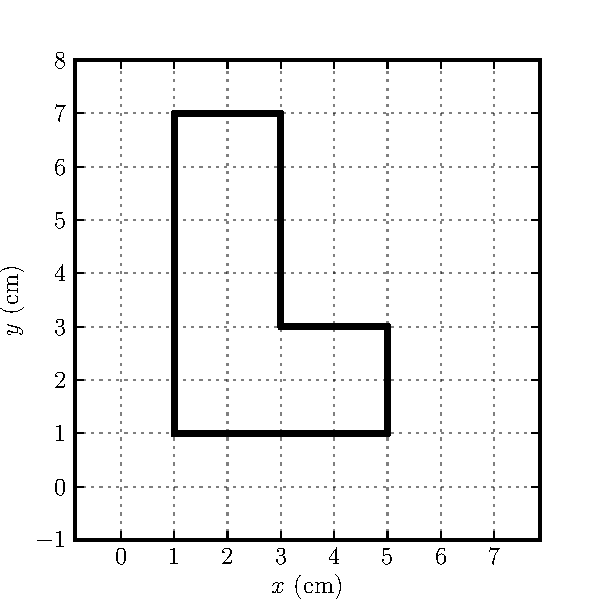
\includegraphics{../py/com_shape.pdf}\\Find the position
of the center of mass of this object, in the given coordinate system;
that is, give the coordinates $(x_\mathrm{cm}, y_\mathrm{cm})$ of the
center of mass.  If you want practice, think up four qualitatively
different ways of doing the center-of-mass calculation.

\paragraph{Problem~\theproblem:}\refstepcounter{problem}%
In the bridge pictured here, identify which beams are under
\emph{tension} stress, and which beams are under \emph{compression}
stress.\\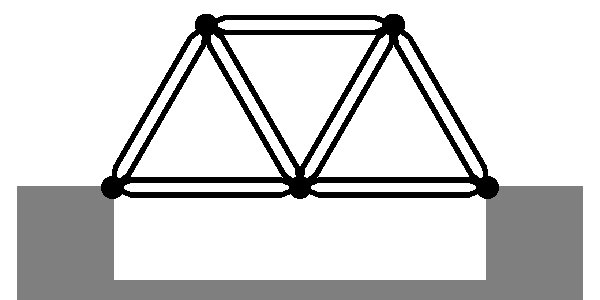
\includegraphics{../py/bridge.pdf}\\ Treat the pins in the
bridge (black dots) as if they are frictionless rotating bearings or
joints.  Treat the entire bridge as if it were resting gently on top
of the ground (that is, the ground is not pulling or pushing
horizontally on the lower-left or lower-right pins).

\paragraph{Problem~\theproblem:}\refstepcounter{problem}%
A typical adult man is holding his left arm at a right angle, so the
upper arm is pointing straight down, and the forearm is pointing
horizontally forwards.  His hand is oriented palm-up.  He is holding a
$20\,\kg$ grocery bag by its handle in his left hand.  Look up the
point of attachment of the relevant tendon and make sensible estimates
(or look them up) for all lengths and masses.  In what follows, treat
the ``hand plus forearm'' to be one monolithic object; that is, we
primarily want to understand the forces at or near the elbow.

\textsl{(a)} Draw a free-body diagram for the hand-plus-forearm
system, identifying all significant forces acting on it (including
from the bag handle, and don't forget the elbow joint---the contact
force from the upper arm bones).

\textsl{(b)} Compute the magnitudes and directions of all forces, and
the magnitudes and directions of all torques, taking the elbow to be
the axis of rotation (that is, the origin or reference point).  For
simplicity, take the tendon direction and joint contact force both to
be precisely vertical.  That is, treat all angles as being right
angles.  This is not a bad approximation.

\textsl{(c)} Look up the definition of ``mechanical advantage'' and
compute the mechanical advantage the grocery bag has over the tendon.
Why would evolution (such a brilliant designer) decide to put tendons
under this kind of stress?

\end{document}
